\documentclass[a4paper,10pt, english]{article}

\usepackage{amssymb}
\usepackage{amsmath}
\usepackage{enumitem}
\usepackage{graphicx}





\newcommand{\D}{\displaystyle}

\newtheorem{theo}{Theorem}[section]
\newcommand{\R}{\mathbb{R}}



\newtheorem{prop}[theo]{Proposition}


\begin{document}

\tableofcontents
\newpage

\section{Some facts about the system}

Consider the dynamical system 

\begin{equation}
\label{s1}
\D
\dot{x_i} = x_i \left(\prod_{j=1}^{N} \left(\frac{x_j}{x_i}\right)^{v_{ij}} - \prod_{j=1}^{N}\left(\frac{x_j}{x_i}\right)^{w_{ij}} \right), \qquad i=1,\ldots, N,
\end{equation}
$$
x_i(0) = x_{i0}, \quad \mbox{\---} \quad \mbox{initial conditions. }
$$


In the case when $\mathbf{v} = \{v_{ij}\}_{i,j=1, \ldots, N}$ and $\mathbf{w} = \{w_{ij}\}_{i,j=1, \ldots, N}$ are stochastic matrices, meaning $\sum_{j=1}^{N}v_{ij} = \sum_{j=1}^{N}w_{ij} = 1$ the system (\ref{s1}) becomes
\begin{equation}
\label{s2}
\D
\dot{x_i}  = \prod_{j=1}^{N} \left(x_j\right)^{v_{ij}} - \prod_{j=1}^{N}\left(x_j\right)^{w_{ij}} , \qquad i=1,\ldots, N.
\end{equation}
The above dynamical system (\ref{s2}) has an equilibrium when
\begin{equation}
\label{s3}
\D
 \prod_{j=1}^{N} \left(x_j\right)^{v_{ij}} - \prod_{j=1}^{N}\left(x_j\right)^{w_{ij}}  = 0, \qquad i=1,\ldots, N.
\end{equation}

Taking the logarithm of (\ref{s3}) and denoting $y_i = \lg{x_i}$, $\Delta_{ij} = v_{ij} - w_{ij}$ the system (\ref{s3}) transforms to the following

\begin{equation}
\label{s4}
\D
\sum_{j=1}^{N}\Delta_{ij}y_j = 0, \qquad i=1,\ldots, N.
\end{equation}

Therefore, (\ref{s3}) holds if  (\ref{s4}) holds. Clearly, (\ref{s4}) holds for $y=(y_1, y_2, \ldots, y_N) = (0, 0, \ldots, 0)$, i.e. the sytem (\ref{s2}) has an equilibrium in 
$x=(x_1, x_2, \ldots, x_N) = (1, 1, \ldots, 1)$. Other equilibrium points are only possible when the matrix $\mathbf{\Delta} = \{\Delta_{ij}\}_{i,j=1, \ldots, N}$ is singular.
Which is true when matrices $\mathbf{v}$ and $\mathbf{w}$ are stochastic, since adding up all the columns in $\mathbf{\Delta}$ will result in a zero column.
Note that for a singular matrix $\mathbf{\Delta}$ there are infinitely many equilibriums, because there are infinitely many solutions of the system (\ref{s4}). 
Let's find those equilibriums. Apart of  $x = (0, 0, \ldots, 0)$ and $x = (1, 1, \ldots, 1)$ (\ref{s3}) holds for $x_1 =  x_2 = \ldots = x_N$ because then (\ref{s3}) become
$$
\D
 x^1 - x^1 = 0, \qquad i=1,\ldots, N.
$$
where $x = x_i$, $\forall i=1,\ldots, N$.

Therefore, the equilibriums of the system (\ref{s2}) constitute a susbpace $U_e\subset\mathbb{R}^N$, $U_e = \{x = (x_1, x_2, \ldots, x_N)\in\mathbb{R}^N | x_1 =  x_2 = \ldots = x_N = x^e\in\mathbb{R}\}$.


\newpage
Let's look at the nature of those equilibriums. The linearization of the system around a poin $x\in U_e$ has the form
$$
\dot{\delta x} = \Delta f(x) \delta x,
$$
where $\D \Delta f(x) = \frac{\partial f_i(x)}{\partial x_j}$, $i, j =1, 2, \ldots, N.$

$$
\frac{\partial f_i(x)}{\partial x_j} = v_{ij}x^{v_{ij}-1}\prod_{k=1, k\neq j}^{N}x^{v_{ik}} - w_{ij}x^{w_{ij}-1}\prod_{k=1, k\neq j}^{N}x^{w_{ik}} =
$$
$$
v_{ij}x^{\sum_{k=1}^{N}v_{ik} - 1} - w_{ij}x^{\sum_{k=1}^{N}w_{ik} - 1} = v_{ij} - w_{ij} = \Delta_{ij},
$$
therefore,  $\Delta f(x) = \mathbf{\Delta}$ for all $x\in U_e$.
\\\\
Note that the matrix $\mathbf{\Delta}$ has always a zero eignvalue, because $|\mathbf{\Delta}| = 0$ therefore, the linearization fails to determine the stability of the equilibrium point. We can only tell the unstability
of the equilibrium i.e. when there exists an eigenvalue of $\mathbf{\Delta}$ with the real larger than 0.
Nevertheless, in our simulations whenever $Re\lambda_i \leq 0$ for all $i$ and for some $i$ $Re\lambda_i = 0$ the solutions seems always to converge asymptotically to some equilibrium in $U_e$ (see Example 1).
The \textquotedblleft purely \textquotedblright stable equilibrium, wich is not asymptotically stable  was observed when all the eigenvalues of $\mathbf{\Delta}$ had zero real parts (see Example 3).

\newpage
\section{Numerical observations}
\subsection{Example 1. Converging pattern}


Consider the case $N=3$, the time horizon $T = 100$,


\[\mathbf{v} =  \left( \begin{array}{ccc}
0 & 0.5 & 0.5 \\
0.5 & 0 & 0.5 \\
0.5 & 0.5 & 0 
\end{array} \right),
%
\mathbf{w} = 
\left( \begin{array}{ccc}
0.5 & 0.5 & 0 \\
0 & 0.5 & 0.5 \\
0.5 & 0 & 0.5 
\end{array} \right),
\]

$$
\mathbf{\Delta} = 
\left(
\begin{matrix}
-0.5   & 0 & 0.5 \\
0.5 &  -0.5 & 0 \\
0 &  0.5 & -0.5 \\
\end{matrix}
\right).
$$
%Here $\mathbf{v}$ and $\mathbf{w}$ are stochastic, then $|\mathbf{\Delta}| = 0$. Therefore the problem has more than one equilibrium. 
The real parts of egenvalues of $\mathbf{\Delta}$ are less or equal zero, namely $Re\lambda_1 = -0.75$,  $Re\lambda_2 = -0.75$, and $Re\lambda_3 = 0$.
Let us have a look at the graph of the solution with the initial conditions $x_0 = (0.3\quad 0.6\quad 0.9)$.

\begin{figure}[ht]
\label{fig_c1}
\centering
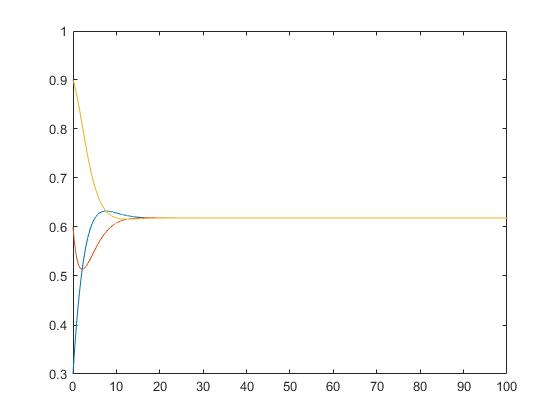
\includegraphics[scale=0.4]{1.jpg}
\caption{$x_0 = (0.3 \quad0.6\quad 0.9)$, $x^e = 0.6184178227652$}.
\end{figure}

The equilibrium  $U_e\ni x^e = 0.6184178227652$.




\newpage
If we change the initial conditions slightly the equilibrium point also changes. For example for the initial conditions
$x_0 = (0.35\quad 0.6\quad 0.9)$ the solutions converge to a different  equilibrium $U_e\ni x^e = 0.635643409191$
\begin{figure}[ht]
\label{fig_c2}
\centering
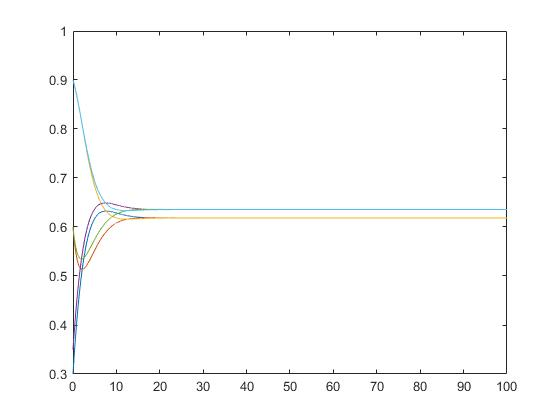
\includegraphics[scale= 0.4]{2.jpg}

\caption{$x_0 = (0.35 \quad0.6\quad 0.9)$, $x^e = 0.635643409191$}
\end{figure}
In (Fig. 2) the two solutions are plotted together for comparison.
In this case it looks like the solutions converge assymptotically.

For the four dimensional case the same behaviour was observed. 



\newpage


\subsection{Example 2. Diverging pattern and the cutoff}
In case  $\mathbf{\Delta}$ has eigenvalues with positive real parts the equilibriums  $U_e$ are not stable and the solutions diverge. Consider for example $N=3$, $T=10$ and the following matrices

\[\mathbf{v} =  \left( \begin{array}{ccc}
 0.5& 0& 0.5\\ 
 0.5 &0.5 &0\\
 0& 0.5& 0.5\\
\end{array} \right),
%
\mathbf{w} = 
\left( \begin{array}{ccc}
0.5& 0.5& 0\\ 
0.5 &0 &0.5\\ 
0.5& 0& 0.5\\
\end{array} \right),
\]

$$
\mathbf{\Delta} = 
\left(
\begin{matrix}
0   & -0.5 & 0.5 \\
0 &  0.5 & -0.5 \\
-0.5 &  0.5 & 0 \\
\end{matrix}
\right).
$$
The real parts of egenvalues of $\mathbf{\Delta}$ are  $Re\lambda_1 = 0.25$,  $Re\lambda_2 = 0.25$, and $Re\lambda_3 = 0$ therefore, the equilibriums 
$U_e$ are not stable. The solutions for the initial condition $x_0 = (0.3\quad 0.6\quad 0.9)$ can be seen on the figure below. 
\begin{figure}[ht]
\label{fig_osc}
\centering
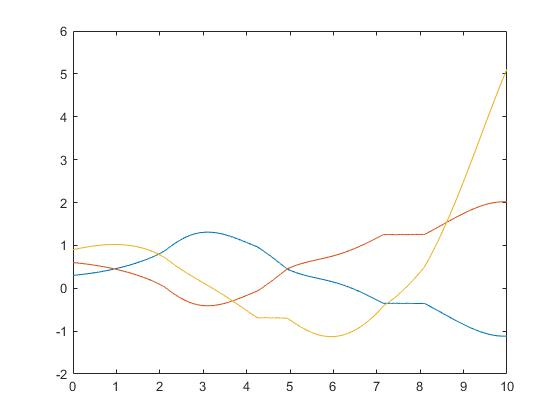
\includegraphics[scale= 0.4]{explode.jpg}
\caption{Solutions diverge}
\end{figure}

At this point it is usefull to consider the cutoff factor $\phi(x) = x(x_{max} - x)$ in (\ref{s1})  to make the solutions stay within the required corridor. The solutions with the cutoff for $T=100$, $x_{max} = 1$ are plotted at the following figure
\begin{figure}[ht]
\label{fig_osc}
\centering
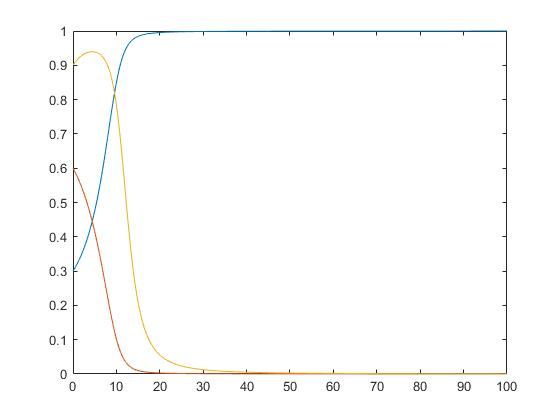
\includegraphics[scale= 0.4]{cutoff.jpg}
\caption{Solutions remain within the [0, 1] corridor.}
\end{figure}







\newpage
\newpage
\newpage
\subsection{Example 3. Oscilating pattern}
For $N=3$, $T=100$ and the matrices

\[\mathbf{v} =  \left( \begin{array}{ccc}
 0.5 & 0   & 0.5 \\
 0.5 & 0.5 & 0   \\
 0   & 0.5 & 0.5 \\
\end{array} \right),
%
\mathbf{w} = 
\left( \begin{array}{ccc}
0.5 & 0.5 & 0\\ 
0  & 0.5 & 0.5\\
0.5 & 0 & 0.5\\
\end{array} \right),
\]

$$
\mathbf{\Delta} = 
\left(
\begin{matrix}
0   & -0.5 & 0.5 \\
0.5 &  0 & -0.5 \\
-0.5 &  0.5 & 0 \\
\end{matrix}
\right)
$$
all the real parts of eigenvalues of $\mathbf{\Delta}$ are zeros. 
The solutions remain bounded within some corridor and oscilate infinitely, which exibits a stable behaviour of the equilibrium. The solutions for the initial condition $x_0 = (0.3\quad 0.6\quad 0.9)$ can be seen on the figure below. 

\begin{figure}[ht]
\label{fig_osc}
\centering
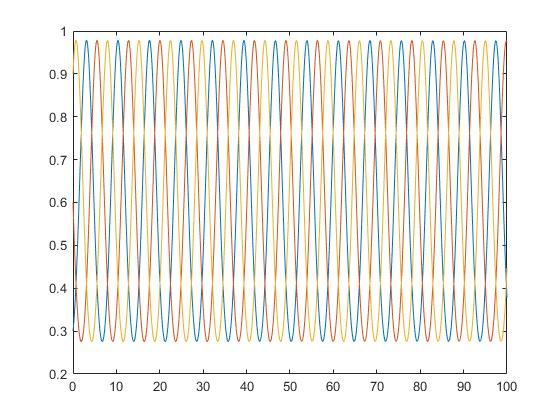
\includegraphics[scale= 0.4]{osc.jpg}
\caption{Oscilatory behavior}
\end{figure}



\newpage
\newpage
\newpage
\subsection{Example 4. Diverging-converging pattern}
We can also consider matrices $\mathbf{v}$ and $\mathbf{w}$ that vary with time. For example we can construct them so that they switch with time from \textquotedblleft bad \textquotedblright to  \textquotedblleft good \textquotedblright  matrices.
By  \textquotedblleft bad \textquotedblright  $\mathbf{v}$ and $\mathbf{w}$  we mean such  matrices that $\mathbf{\Delta}$ has positive real parts of eignvalues, and  \textquotedblleft good \textquotedblright  matrices are such that $\mathbf{\Delta}$ has all real parts of eigenvalues less or equal zero.

Consider the following matrices $\mathbf{v}(t) = \lambda(t)\mathbf{v_g} + (1-\lambda(t))\mathbf{v_b}$ and  $\mathbf{w}(t) = \lambda(t)\mathbf{w_g} + (1-\lambda(t))\mathbf{w_b}$, where $\mathbf{v}_g$, $\mathbf{w}_g$, and $\mathbf{v}_b$, $\mathbf{w}_b$ are good and bad matrices respectively,
$$
\lambda(t) = \frac{t}{\gamma T}, \qquad 0<t\leq T, \quad 0<\gamma<1.
$$
Then, we have that the bad matrices switch smoothly to the good matrices in time $\gamma T$.
For example, choose the good matrices from the Example 1 and bad matrices from the Example 2. For $N=3$, $T=300$, $x_0 = (0.3\quad 0.6\quad 0.9)$ and cutoff term $\phi(x) = x(x_{max} - x)$, $x_{max} = 1$ the solutions are plotted at the following figure


\begin{figure}[ht]
\label{fig_c4}
\centering
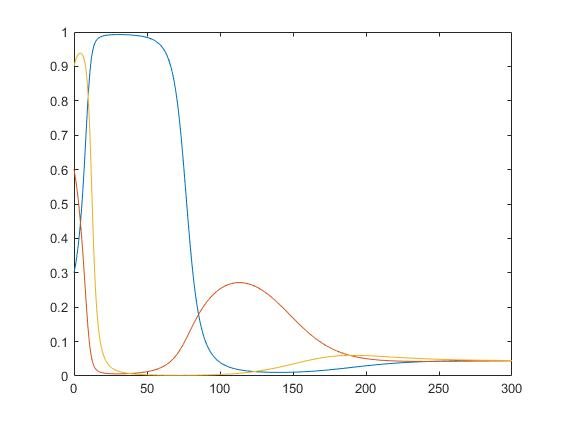
\includegraphics[scale= 0.4]{switch.jpg}
\caption{Trajectories switch from diverging to converging.}
\end{figure}
As matrices switch from bad to good ones the behaviour of the trajectories switches from diverging to converging.





\newpage
\newpage
\newpage
\subsection{Example 5. Equilibrium space visualization}
To picture how the equilibrium space looks like, consider a two dimensional case  $N=2$, and let us plot the phase portrait of the system (\ref{s2}), for the time horizon $T = 10$. and

\[\mathbf{v} =  \left( \begin{array}{cc}
0 & 0.5  \\
0.5 & 0 \\
\end{array} \right),
%
\mathbf{w} = 
\left( \begin{array}{cc}
0.5 & 0 \\
0 & 0.5 \\
\end{array} \right),
\]


$$
\mathbf{\Delta} = 
\left(
\begin{matrix}
-0.5 & 0.5 \\
0.5 & -0.5 \\
\end{matrix}
\right).
$$


\begin{figure}[ht]
\label{fig_c3}
\centering
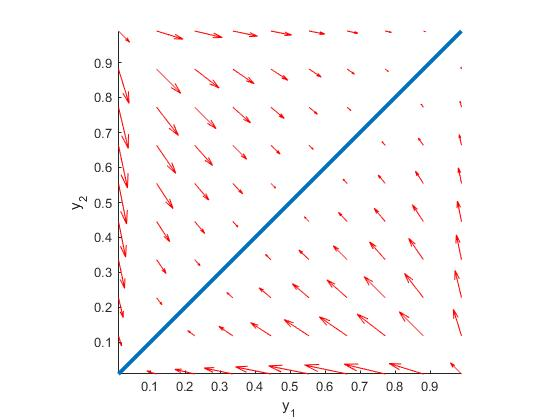
\includegraphics[scale= 0.4]{3.jpg}
\caption{Phase portrait}
\end{figure}
Here in  (Fig. 3) the thick bisectrice is the equilibrium space $U_e$, and and the red arrows show where the trajectories tend with time.
The trajectories along with the phase portrait are plotted on the following (Fig. 4)
\begin{figure}[ht]
\label{fig_c4}
\centering
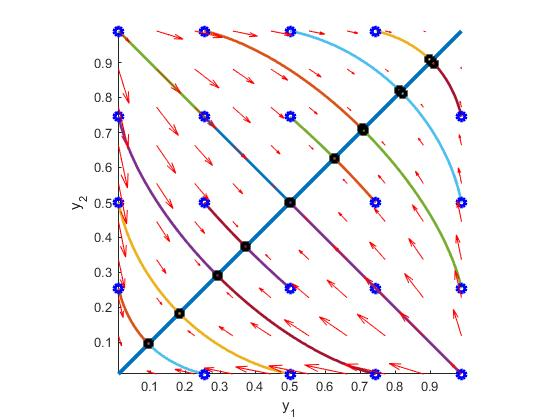
\includegraphics[scale= 0.4]{4.jpg}
\caption{Phase portrait along with the trajedivergectories}
\end{figure}
where the blue circles denote the beginning of the trajectories and the dark squares denote the end of the trajectories.
The trajectory portrait in the $3-dim$ case in the first example is pictured on the following figure
\begin{figure}[ht]
\label{fig_c4}
\centering
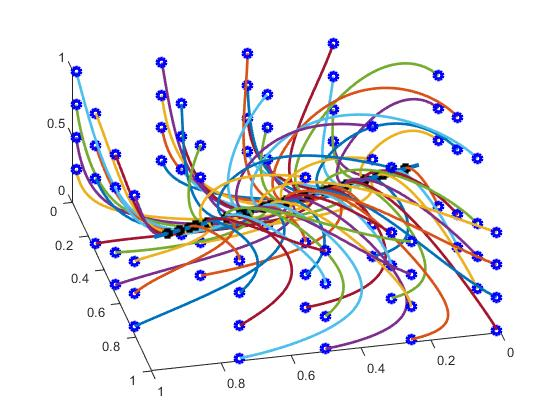
\includegraphics[scale= 0.4]{5.jpg}
\caption{Trajectory portrait.}
\end{figure}
As can be seen all trajectories converge to the bisectrice of the first cuboid.



\end{document}
